%!TEX root = index.tex
\chapter[Revisão Bibliográfica]{Revisão Bibliográfica}
\label{chap:revisao}
\section{Parceria Universidade-Empresa}
\label{cha:ensino}
\subsection{A universidade empreendedora}
\label{cha:univ_empreend}

Ao longo da história as universidades sofreram alterações no seu papel diante da visão da sociedade, mudando grande parte de suas características e atividades. Segundo \citeonline{etzkowitz2001}, duas revoluções aconteceram no modelo de funcionamento da universidade.

Como instituições de origem medieval, as universidades tinham como principal objetivo a conservação, preservação e transmissão de sua cultura através das gerações. Conforme o passar dos anos e novas descobertas sendo feitas, surgiram os seminários como principal forma de disseminação de conhecimento, até evoluirem para os modelos de ensino similares aos atuais. Caracteriza-se essa fase anterior as revoluções como centrada no ensino.

A primeira revolução acadêmica ocorre com a evolução dos modelos de ensino e universidades adotando um modelo intenso de pesquisa, com a intenção de promover avanços na ciência. Com a transmissão mais acessível de pequenas novas descobertas, as pesquisas começaram a se basear em pesquisas já realizadas, gerando um ambiente de pesquisa colaborativa. 

Durante e após a Segunda Guerra Mundial nos Estados Unidos, a estrutura de pesquisas começou a receber grandes aportes financeiros, e a equipe de pesquisas começou a crescer de tal forma que foram surgindo necessidades de responsabilidades além das exercidas por alunos e pesquisadores, principalmente em relação à administração dessa estrutura de pesquisas, como manutenção da propriedade intelectual e divulgação de novas descobertas. O ambiente de pesquisas começou a ficar similar a uma empresa, o que levou a segunda revolução da academia.

Com uma estrutura voltada a acelerar o desenvolvimento de pesquisas, os laboratórios passaram a ser vistos como fonte de resolução de problemas reais do mercado. A segunda revolução acadêmica aconteceu quando as universidades passaram a utilizar seus laboratórios de pesquisa para realizar descobertas que pudessem gerar produtos comerciáveis. Desta forma, também foi inserido o desenvolvimento econômico como uma nova missão da universidade, além da pesquisa e do ensino.

Dessa forma, surge o conceito de Universidade Empreendedora, que recebe diferentes concepções de diversos autores. Segundo \citeonline{etzkowitz2001}, é uma instituição que trabalha ativamente na transferência de tecnologia e no desenvolvimento econômico, já para \citeonline{burton} é uma instituição que realiza um esforço contínuo de reformulação institucional de forma a melhorar o desempenho para com empresas e o governo, e para \citeonline{plonsky} é uma instituição que exerce um papel ativo no mercado do conhecimento.

\begin{figure}
\caption{Revoluções Acadêmicas}
\centerline{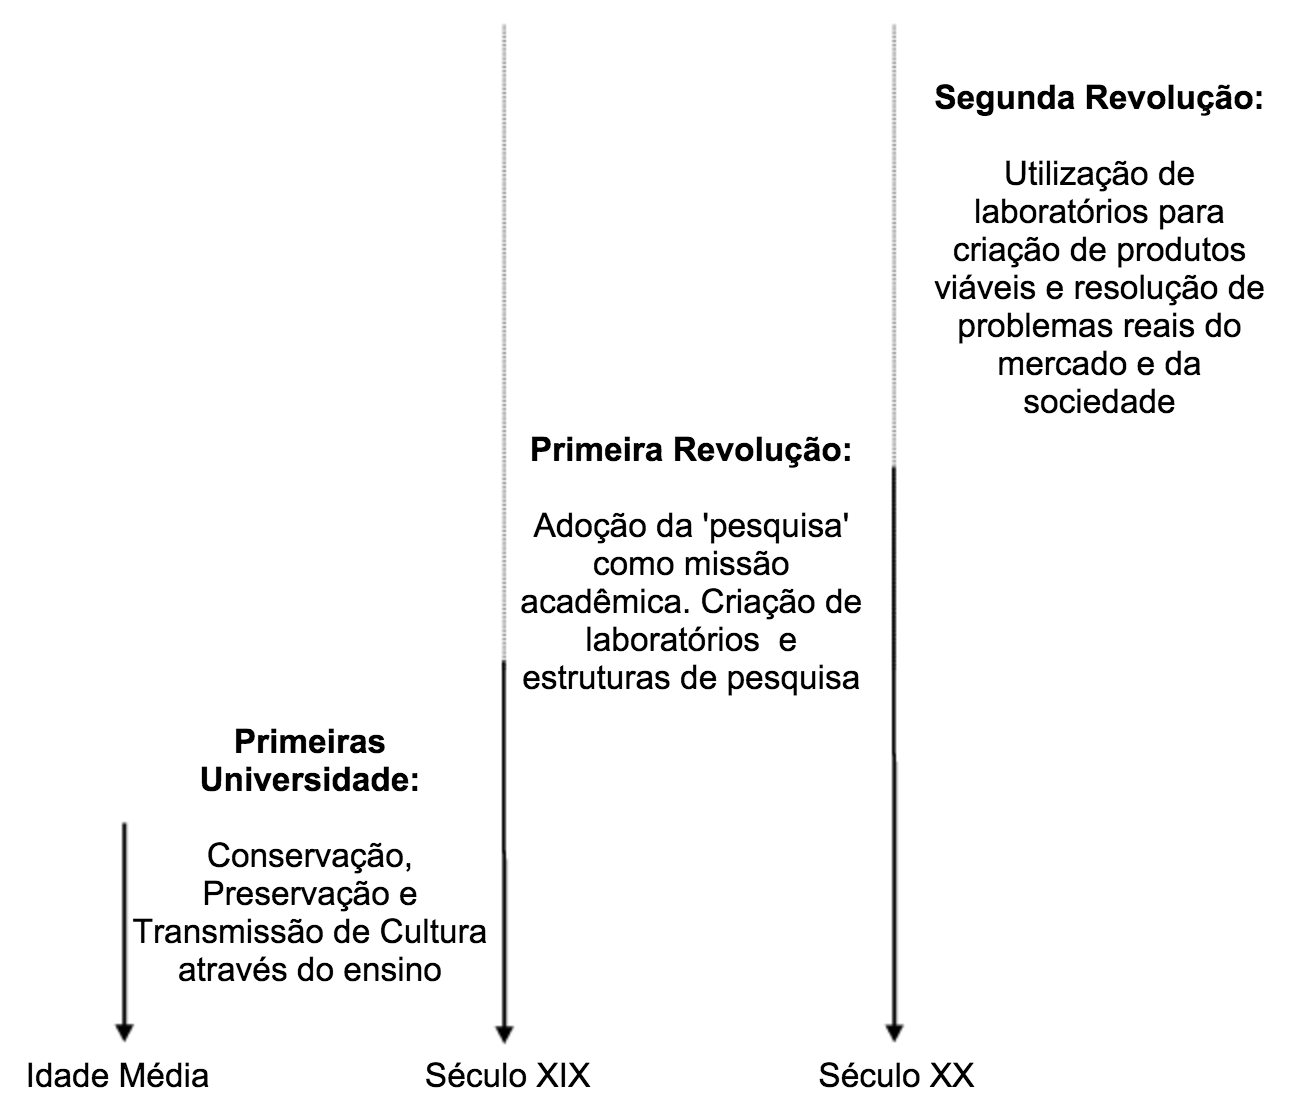
\includegraphics[scale=0.5]{img/academic_revolutions}}
\label{fig:academic_revolutions}
\caption* {Fonte: Elaborado pelo autor a partir de \citeonline{etzkowitz2001}}
\end{figure}



\subsection{Interação universidade-empresa-governo}
\label{cha:univ_empreend}

\begin{figure}[H]
\caption{PRIMEIRO MODELO}
\centerline{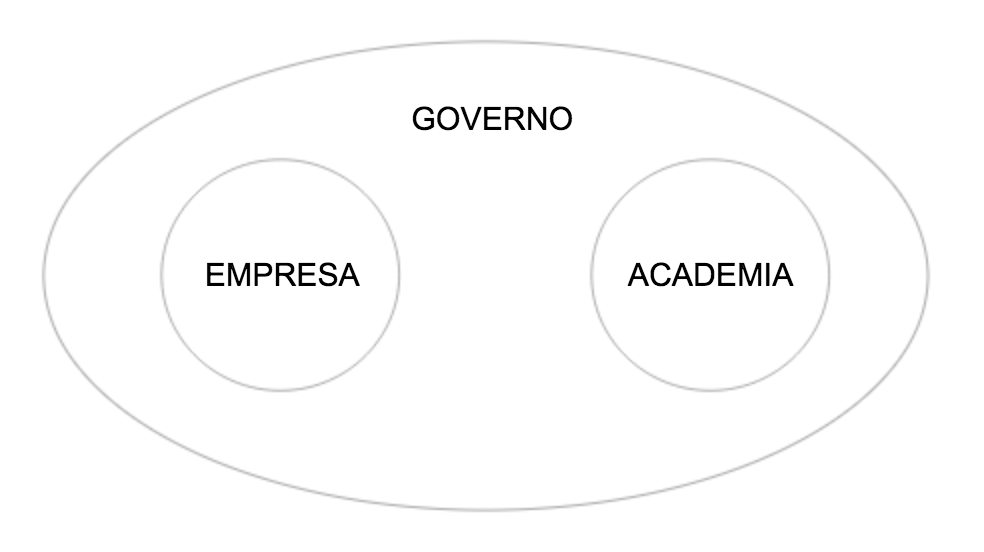
\includegraphics[scale=0.5]{img/triplehelix1}}
\label{fig:triplehelix1}
\caption* {Fonte: \citeonline{etzkowitz2000}}
\end{figure}

\begin{figure}
\caption{SEGUNDO MODELO}
\centerline{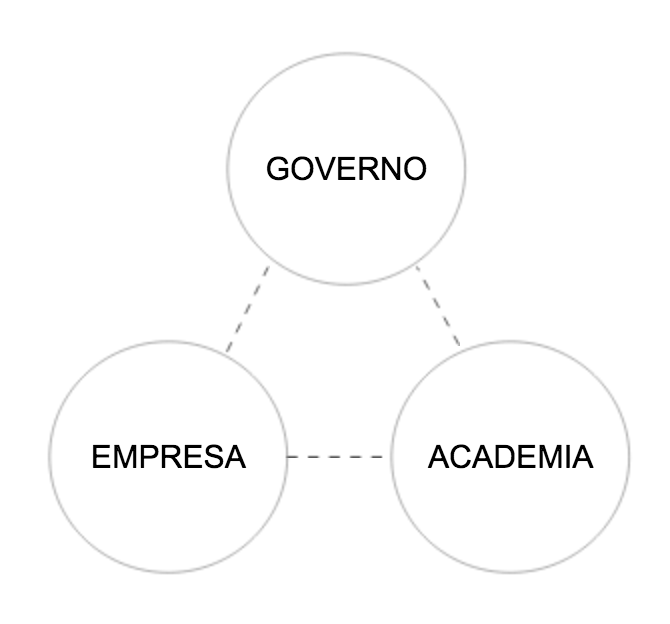
\includegraphics[scale=0.5]{img/triplehelix2}}
\label{fig:triplehelix2}
\caption* {Fonte: \citeonline{etzkowitz2000}}
\end{figure}

\begin{figure}
\caption{TERCEIRO MODELO}
\centerline{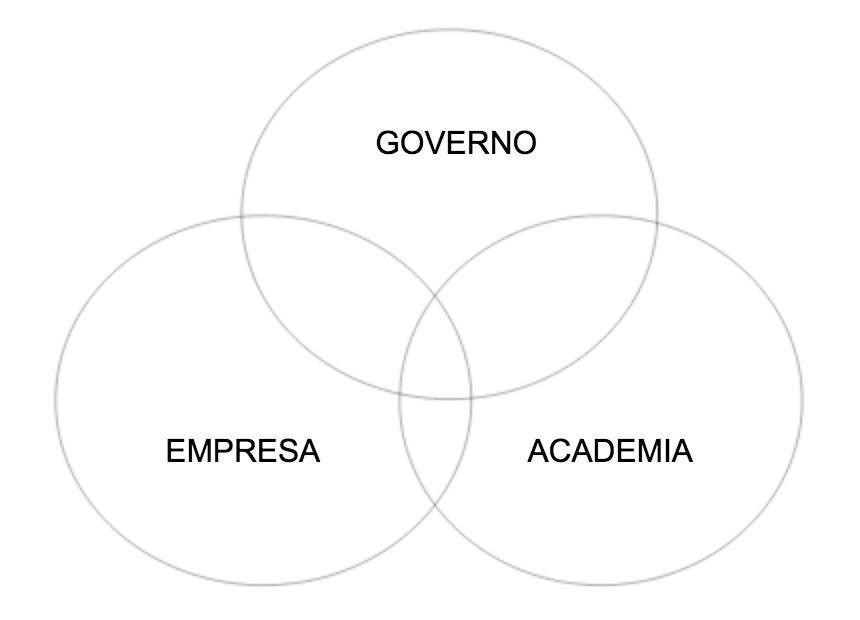
\includegraphics[scale=0.5]{img/triplehelix3}}
\label{fig:triplehelix3}
\caption* {Fonte: \citeonline{etzkowitz2000}}
\end{figure}

\subsection{Desafios da gestão universidade-empresa}
\label{cha:univ_empreend}

Ary Plonski:

"Nos últimos anos, a ênfase da discussão sobre a cooperação entre a academia e o chamado setor produtivo tem-se deslocado da temática ideológica para a da gestão"
"Do lado empresarial, hoje são raras as manifestações, ao menos públicas, de confronto ideológico com a instituição universitária."

"(Dado o alinhamento ideológico entre as partes), um fator crítico para o êxito da cooperação é a gestão adequada da interface em seus vários níveis - desde o alinhamento de percepções dos cooperantes a respeito de quais são os diferentes objetivos colimados com a relação e os condicionantes que cada cultura impõe, até a administração cotidiana dos projetos e atividades envolvidas na transformação dos objetivos estipulados em resultados tangíveis."

"Os artigos apresentados nesta edição da RAUSP permitem identificar e caracterizar alguns dos mais importantes desafios gerenciais para tornar a cooperação empresa-universidade não apenas mutuamente benéfica, mas também uma relação transformadora. Dentre eles, destacam-se os seguintes: 
- compartilhar uma visão multidimensional e integrada da cooperação universidade-empresa, centrada no desenvolvimento de competências humanas

.: A parceria entre a universidade e o setor produtivo dá-se primeiramente no plano de ensino de graduação, com o aproveitamento de quadros profissionais formados pela academia em escalões superiores das empresas. (Gabao - Isso significa que o desenvolvimento de competências para alunos de graduação refletirão em bons profissionais para as empresas, e esse tipo de parceria não envolve algo garantido entre empresa e universidade, mas é um dos exemplos de atuação cooperativa entre ambas as partes, por isso deve-se existir essa visão multidimensional e integrada)

- perceber com clareza as missões distintas, mas complementares, da empresa e da universidade no processo de inovação

.: De um lado estão as universidades empreendedoras (\textit{entrepreneurial universities}). Apresentadas em foros internacionais como um modelo inspirador para a universidade no próximo século	, enfatizam, a par de excelência acadêmica tradicional, um papel ativo da universidade no mercado do conhecimento. De outro lado estão as universidades corporativas (\textit{corporate universities}), entidades criadas por empresas para "formar e desenvolver os talentos humanos na gestão dos negócios", conforme definição apresentada por Marisa Eboli em seu artigo.  Cabe observar, preliminarmente, que não é papel usual da universidade - e sim da empresa - desenvolver tecnologia, entendida como conhecimento organizado aplicável à produção de bens e serviços.

- desenvolver respostas inovativas às diversas necessidades de cooperação empresa-universidade

.: Merecem destaque dois aspectos relevantes dessa experiência para a gestão da cooperação, no contexto da sociedade do conhecimento. O primeiro é que, mesmo em uma relação institucional assimétrica, a verdadeira cooperação envolve aprendizado por ambas as instituições, pois "a Universidade beneficia-se com a compreensão das reais necessidades da sociedade e as empresas passam a ter acesso ao enorme acervo de conhecimentos, sendo beneficiadas com soluções rápidas, além de poderem capacitar-se melhor". 

- capacitar para a gestão eficaz da cooperação empresa-universidade"

.: A gestão adequada da cooperação entre a academia e o segmento produtivo requer conhecimentos, habilidades e atitudes apropriadas para lidar com questões estratégicas - começando pela missão e pela visão institucional - táticas, como a da propriedade intelectual e a do equacionamento econômico-financeiro mais favorável, e operacionais, como a gestão de projetos, frequentemente pluri-institucionais, capazes de transformar desejos em resultados. 

\begin{itemize}
\item Jorge Luis Nicolas Audy
\end{itemize}

"O atuala sistema de financiamento da pesquisa e da Universidade indica a necessidade de uma busca por sustentabilidade nestas atividades de pesquisa e também da própria Universidade por novas fontes de receita."

"A medida que a sociedade vai se tornando mais baseada no conhecimento, as empresas vão mudando suas características e o mercado de trabalho vai setornando mais intensivo em conhecimento, gerando demandas por um novo tipo de profissional. Ao mesmo tempo a sociedade passa a esperar mais das Universidades em termos de contribuições ao processo de desenvolvimento econômico e social. Os problemas se tornam mais complexos e o ambiene mais incerto. Neste contexto, as demandas da sociedade crescem constantemente e a capacidade de responder a estas demandas desequilibra-se."

\section{Metodologia de Entrevistas}
\label{cha:ensino}
